\documentclass[10pt,twocolumn,letterpaper]{article}

% CVPR-style formatting and fonts
\usepackage{cvpr}
\usepackage{times}
\usepackage{epsfig}
\usepackage{graphicx}
\usepackage{amsmath}
\usepackage{amssymb}
\usepackage{url}
\usepackage{siunitx}
\sisetup{group-separator = {\,}, group-minimum-digits=4}
\usepackage{booktabs}
\usepackage{subcaption}
\usepackage{caption}
\captionsetup{compatibility=false}
\usepackage{tabularx}
\usepackage{authblk}

\newcolumntype{Y}{>{\raggedright\arraybackslash}X}

\cvprfinalcopy
\def\cvprPaperID{****}
\def\httilde{\mbox{\tt\raisebox{-.5ex}{\symbol{126}}}}
\ifcvprfinal\pagestyle{empty}\fi

\begin{document}

\title{Parallel Acceleration of Quantum Kernel Methods for Image Classification Tasks: \\ A Detailed Project Report from Unified Pipelines to CUDA Debugging}

\author{Fouepe Dylan\\
{\tt\small dylan.fouepe@edu.unifi.it}}
\affil{University of Florence}

\maketitle
\thispagestyle{empty}

\begin{abstract}
This project studies training binary SVMs on classical image datasets using simulated quantum kernels, with a strong focus on parallel programming and heterogeneous CPU/GPU optimization. The repository provides three coherent execution paths: a classical CPU baseline, a GPU quantum backend based on PennyLane+PyTorch (\texttt{torch}), and a custom HPC backend (\texttt{cuda\_states}) built on CuPy, DLPack and a bespoke C++ CUDA kernel. The scientific core of the work is to build quantum Gram matrices of size $N \times N$ quickly and correctly, whose cost remains $O(N^2 \cdot 2^Q)$ for $Q$ qubits.

The evaluation emphasizes measurable outcomes rather than implementation details: throughput, runtime, F1, AUC, and kernel-shape diagnostics. Results are reported with run-scoped extraction to avoid mixing historical logs and to preserve comparability across backends.

Experiments on Fashion-MNIST, CIFAR-10 and SVHN reveal two regimes. On Fashion-MNIST the quantum kernel remains strong in the latest run-scoped campaign, with best values up to \textbf{F1 = 0.9653} and \textbf{AUC = 0.9956} (\texttt{torch}, size 1000). On CIFAR-10 and SVHN, however, kernels tend to concentrate, the inter-class gap becomes nearly zero, and the SVM often ends with a support-vector fraction close to $1.0$, consistent with a \emph{kernel collapse} or \emph{barren-plateau-like} behavior. Overall, the reported results provide a consistent comparison of throughput and predictive quality across classical and quantum-kernel settings.
\end{abstract}

\section{Introduction}
Quantum kernel methods provide a clean way to project classical data into a very high-dimensional Hilbert space and then solve a classification task with a precomputed SVM~\cite{havlicek2019supervised}. In practice this promise quickly runs into a cost problem: for $N$ samples and $Q$ qubits, building the Gram matrix requires simulating states of dimension $2^Q$ and evaluating $O(N^2)$ complex overlaps. At $Q=16$ a single state vector already contains $65{,}536$ complex amplitudes.

The study compares a classical SVM baseline and two quantum-kernel backends under the same experimental protocol. The report focuses on comparative evidence: predictive quality (F1/AUC), runtime, throughput, and failure indicators related to kernel concentration.

\section{Scope of the Project}
This study addresses three questions:
\begin{itemize}
    \item How do classical and quantum-kernel SVMs compare on the same binary tasks?
    \item Which backend offers the best throughput-runtime trade-off at 16 qubits?
    \item Which empirical signals indicate kernel concentration and loss of separability?
\end{itemize}

The analysis focuses on measurable outcomes: F1, AUC, runtime, throughput, and kernel-shape diagnostics.

\section{Experimental Methodology}
Three datasets are used for binary classification: Fashion-MNIST~\cite{xiao2017fashion}, CIFAR-10~\cite{krizhevsky2009cifar}, and SVHN~\cite{netzer2011svhn}. Each is binarized into three tasks of increasing difficulty (see Table~\ref{tab:tasks}). All experiments use $Q=16$ qubits by default, yielding state vectors of dimension $2^{16} = 65{,}536$ complex amplitudes. Key performance observations from the benchmark campaign at this scale are:
\begin{itemize}
    \item for heavy cases at 16 qubits, \texttt{cuda\_states} becomes significantly faster than the CPU backend;
    \item at 10,000 samples, the speedup is already about $2.5\times$;
    \item at 30,000 samples, the speedup exceeds $4.8\times$;
    \item the observed VRAM peak reaches approximately \SI{29.3}{GB} for \texttt{cuda\_states} at 30,000 samples.
\end{itemize}

\begin{table}[t]
\centering
\caption{Binary classification tasks configured in the repository.}
\label{tab:tasks}
\small
\begin{tabular}{llll}
\toprule
\textbf{Dataset} & \textbf{Easy} & \textbf{Med} & \textbf{Hard} \\
\midrule
Fashion-MNIST & 0 vs 1 & 3 vs 8 & 0 vs 6 \\
CIFAR-10 & 1 vs 6 & 0 vs 2 & 3 vs 5 \\
SVHN & 1 vs 0 & 2 vs 7 & 3 vs 5 \\
\bottomrule
\end{tabular}
\end{table}

From the quantum perspective, most configurations use $16$ PCA components (thus $16$ qubits) with a shallow circuit depth by default. Circuit layers are configurable via YAML through \texttt{pennylane.layers}; an important case is \texttt{configs/cifar10\_hard.yaml}, which forces \textbf{6 layers} and serves as a "hard" regime to observe kernel concentration.

\subsection{Preprocessing and Quantum Feature Map}
The training pipeline follows these steps:
\begin{enumerate}
    \item extract pixel values and flatten;
    \item apply PCA to $d=16$ components;
    \item scale features via \texttt{MinMaxScaler};
    \item encode features using the \texttt{angle}, \texttt{ry} or \texttt{ryrz} maps;
    \item simulate states via PennyLane/\texttt{lightning}.
\end{enumerate}

The experiments use the \texttt{RYRZ} ansatz with entangling layers, which provides a simple trade-off between expressivity and simulation cost. Circuit weights are initialized once per run from a normal distribution and kept fixed during SVM training; this is therefore not a full variational training loop but a \emph{kernel-based} learning approach.

The target kernel is the fidelity kernel
\[
k(x_i, x_j) = \left|\langle \psi(x_i) \mid \psi(x_j) \rangle \right|^2.
\]
In practice, if $S_A \in \mathbb{C}^{N_A \times 2^Q}$ and $S_B \in \mathbb{C}^{N_B \times 2^Q}$ are the state matrices, then
\[
K_{ij} = \left| \sum_{k=1}^{2^Q} S_A[i,k]\;\overline{S_B[j,k]} \right|^2.
\]

\subsection{Training Protocol}
The experimental protocol uses:
\begin{itemize}
    \item train/test split inherited from the dataset;
    \item 3-fold cross-validation on the training partition;
    \item hyperparameter optimization of $C$ via Optuna~\cite{akiba2019optuna};
    \item final re-fit on train+val;
    \item final evaluation on the test set.
\end{itemize}

In addition to F1 and AUC, the analysis tracks runtime, support-vector fraction, and kernel distribution statistics to distinguish optimization effects from representational limits.

\section{HPC Architecture}
\subsection{Unified Backend API}
All Gram computation logic converges to a single function:
\[
\texttt{compute\_kernel\_matrix}(X, Y, \ldots).
\]
This API accepts the same data and normalization flags, but delegates execution to three paths:
\begin{itemize}
    \item \texttt{numpy}: CPU fallback, useful as a reference and for small cases;
    \item \texttt{torch}: generate states and perform matrix computation directly on the GPU with PyTorch;
    \item \texttt{cuda\_states}: generate states with PyTorch, convert tensors to CuPy via DLPack, and compute the Gram with a custom \texttt{RawKernel}.
\end{itemize}

\subsection{Torch GPU Backend}
The \texttt{torch} backend uses native PyTorch GPU operations to generate states and compute Gram matrices. In this study it is treated as the main GPU reference point for quality/runtime comparison against both \texttt{numpy} and \texttt{cuda\_states}.

\subsection{Custom CUDA Backend \texttt{cuda\_states}}
The \texttt{cuda\_states} backend computes Gram matrices with custom CUDA kernels through CuPy. In this report, its role is assessed by measured throughput and downstream classification metrics, not by internal kernel structure.

All backend comparisons use the same post-processing and evaluation protocol to preserve metric comparability.

\subsection{Memory Management, Tiling, and Streams}
The benchmark explores the following runtime controls:
\begin{itemize}
    \item \textbf{VRAM-aware sizing}: \texttt{state\_tile=-1} automatically sizes state block dimensions according to available VRAM.
    \item \textbf{Autotuning}: CUDA kernel tile sizes are learned and cached in \texttt{.cuda\_kernel\_autotune.json}. A specific entry for 16 qubits in double precision is handled.
    \item \textbf{Bulk precompute}: when memory permits, all states in a block are prebuilt to reduce round-trips.
    \item \textbf{Stream pool}: multiple CUDA streams can be used to orchestrate state preparation and Gram computation.
    \item \textbf{Memory profiling}: the benchmark measures VRAM usage, transfers and throughput.
\end{itemize}

In the reported campaign, the observed best settings were \texttt{vram\_fraction=0.95}, \texttt{num\_streams=1}, and \texttt{torch\_pinned+streams} for the torch path.

\subsection{Numerical Safety and Shared Post-Processing}
Cross-backend comparisons use a shared post-processing definition:
\begin{itemize}
    \item finite-value checks (NaN/Inf) before writing kernel blocks;
    \item shared kernel normalization across backends;
    \item strict cross-normalization
    \[
    \hat K(X,Y)_{ij} = \frac{K(X,Y)_{ij}}{\sqrt{K(X,X)_{ii}K(Y,Y)_{jj}}}
    \]
    is applied after computing the diagonals.
\end{itemize}

This common normalization makes the backend comparison interpretable at the metric level.

\section{Validation Protocol}
Validation relies on three measurable checks:
\begin{itemize}
    \item cross-backend consistency checks on normalized kernel blocks;
    \item numerical stability checks (NaN/Inf, diagonal validity, normalization bounds);
    \item run-scoped result extraction to avoid mixing historical logs.
\end{itemize}

These checks separate implementation correctness from model performance and support reproducible comparisons.

\section{Performance Results}
\subsection{Benchmark}
The repository benchmark reports more than a single runtime. It captures qubit scaling, sample scaling, optimization ablations, tile-state tuning, VRAM-fraction sensitivity, stream-count impact, and kernel fidelity against the \texttt{numpy} reference. The latest validated campaign used dataset profiles for Fashion-MNIST, CIFAR-10, and SVHN with two warmup runs and two timed runs per point. Outputs are stored under \texttt{benchmark\_results/fashion/}, \texttt{benchmark\_results/cifar10/}, and \texttt{benchmark\_results/svhn/}, with execution logs under \texttt{benchmark\_results/logs/}.

\begin{table}[t]
\centering
\caption{Essential benchmark statistics from the latest profile sweep (Mpairs/s).}
\label{tab:benchmark}
\small
\begin{tabular}{lcc}
\toprule
\textbf{Dataset} & \textbf{Fastest backend panel} & \textbf{Best overall throughput} \\
\midrule
fashion & \texttt{cuda\_states} 0.088 & \texttt{numpy} 0.101 \\
cifar10 & \texttt{cuda\_states} 0.047 & \texttt{numpy} 0.097 \\
svhn & \texttt{cuda\_states} 0.049 & \texttt{numpy} 0.097 \\
\bottomrule
\end{tabular}
\end{table}

Key observations from these benchmark statistics are:
\begin{itemize}
    \item \texttt{cuda\_states} remains the fastest backend in direct backend-comparison panels on all three datasets.
    \item The best single throughput value in each profile often comes from \texttt{numpy} on easier points (small/medium kernels), showing that CPU remains competitive at this scale.
    \item At sample scaling $N=1024$, \texttt{torch} exceeds \texttt{numpy} on CIFAR-10 and SVHN, while \texttt{numpy} remains ahead on Fashion-MNIST.
\end{itemize}

Taken together, these results indicate a mixed regime: backend-comparison tests favor the custom GPU path, while the absolute best-throughput rows can still be obtained on CPU for moderate configurations.

\begin{figure*}[t]
\centering
\begin{subfigure}[t]{0.32\textwidth}
    \centering
    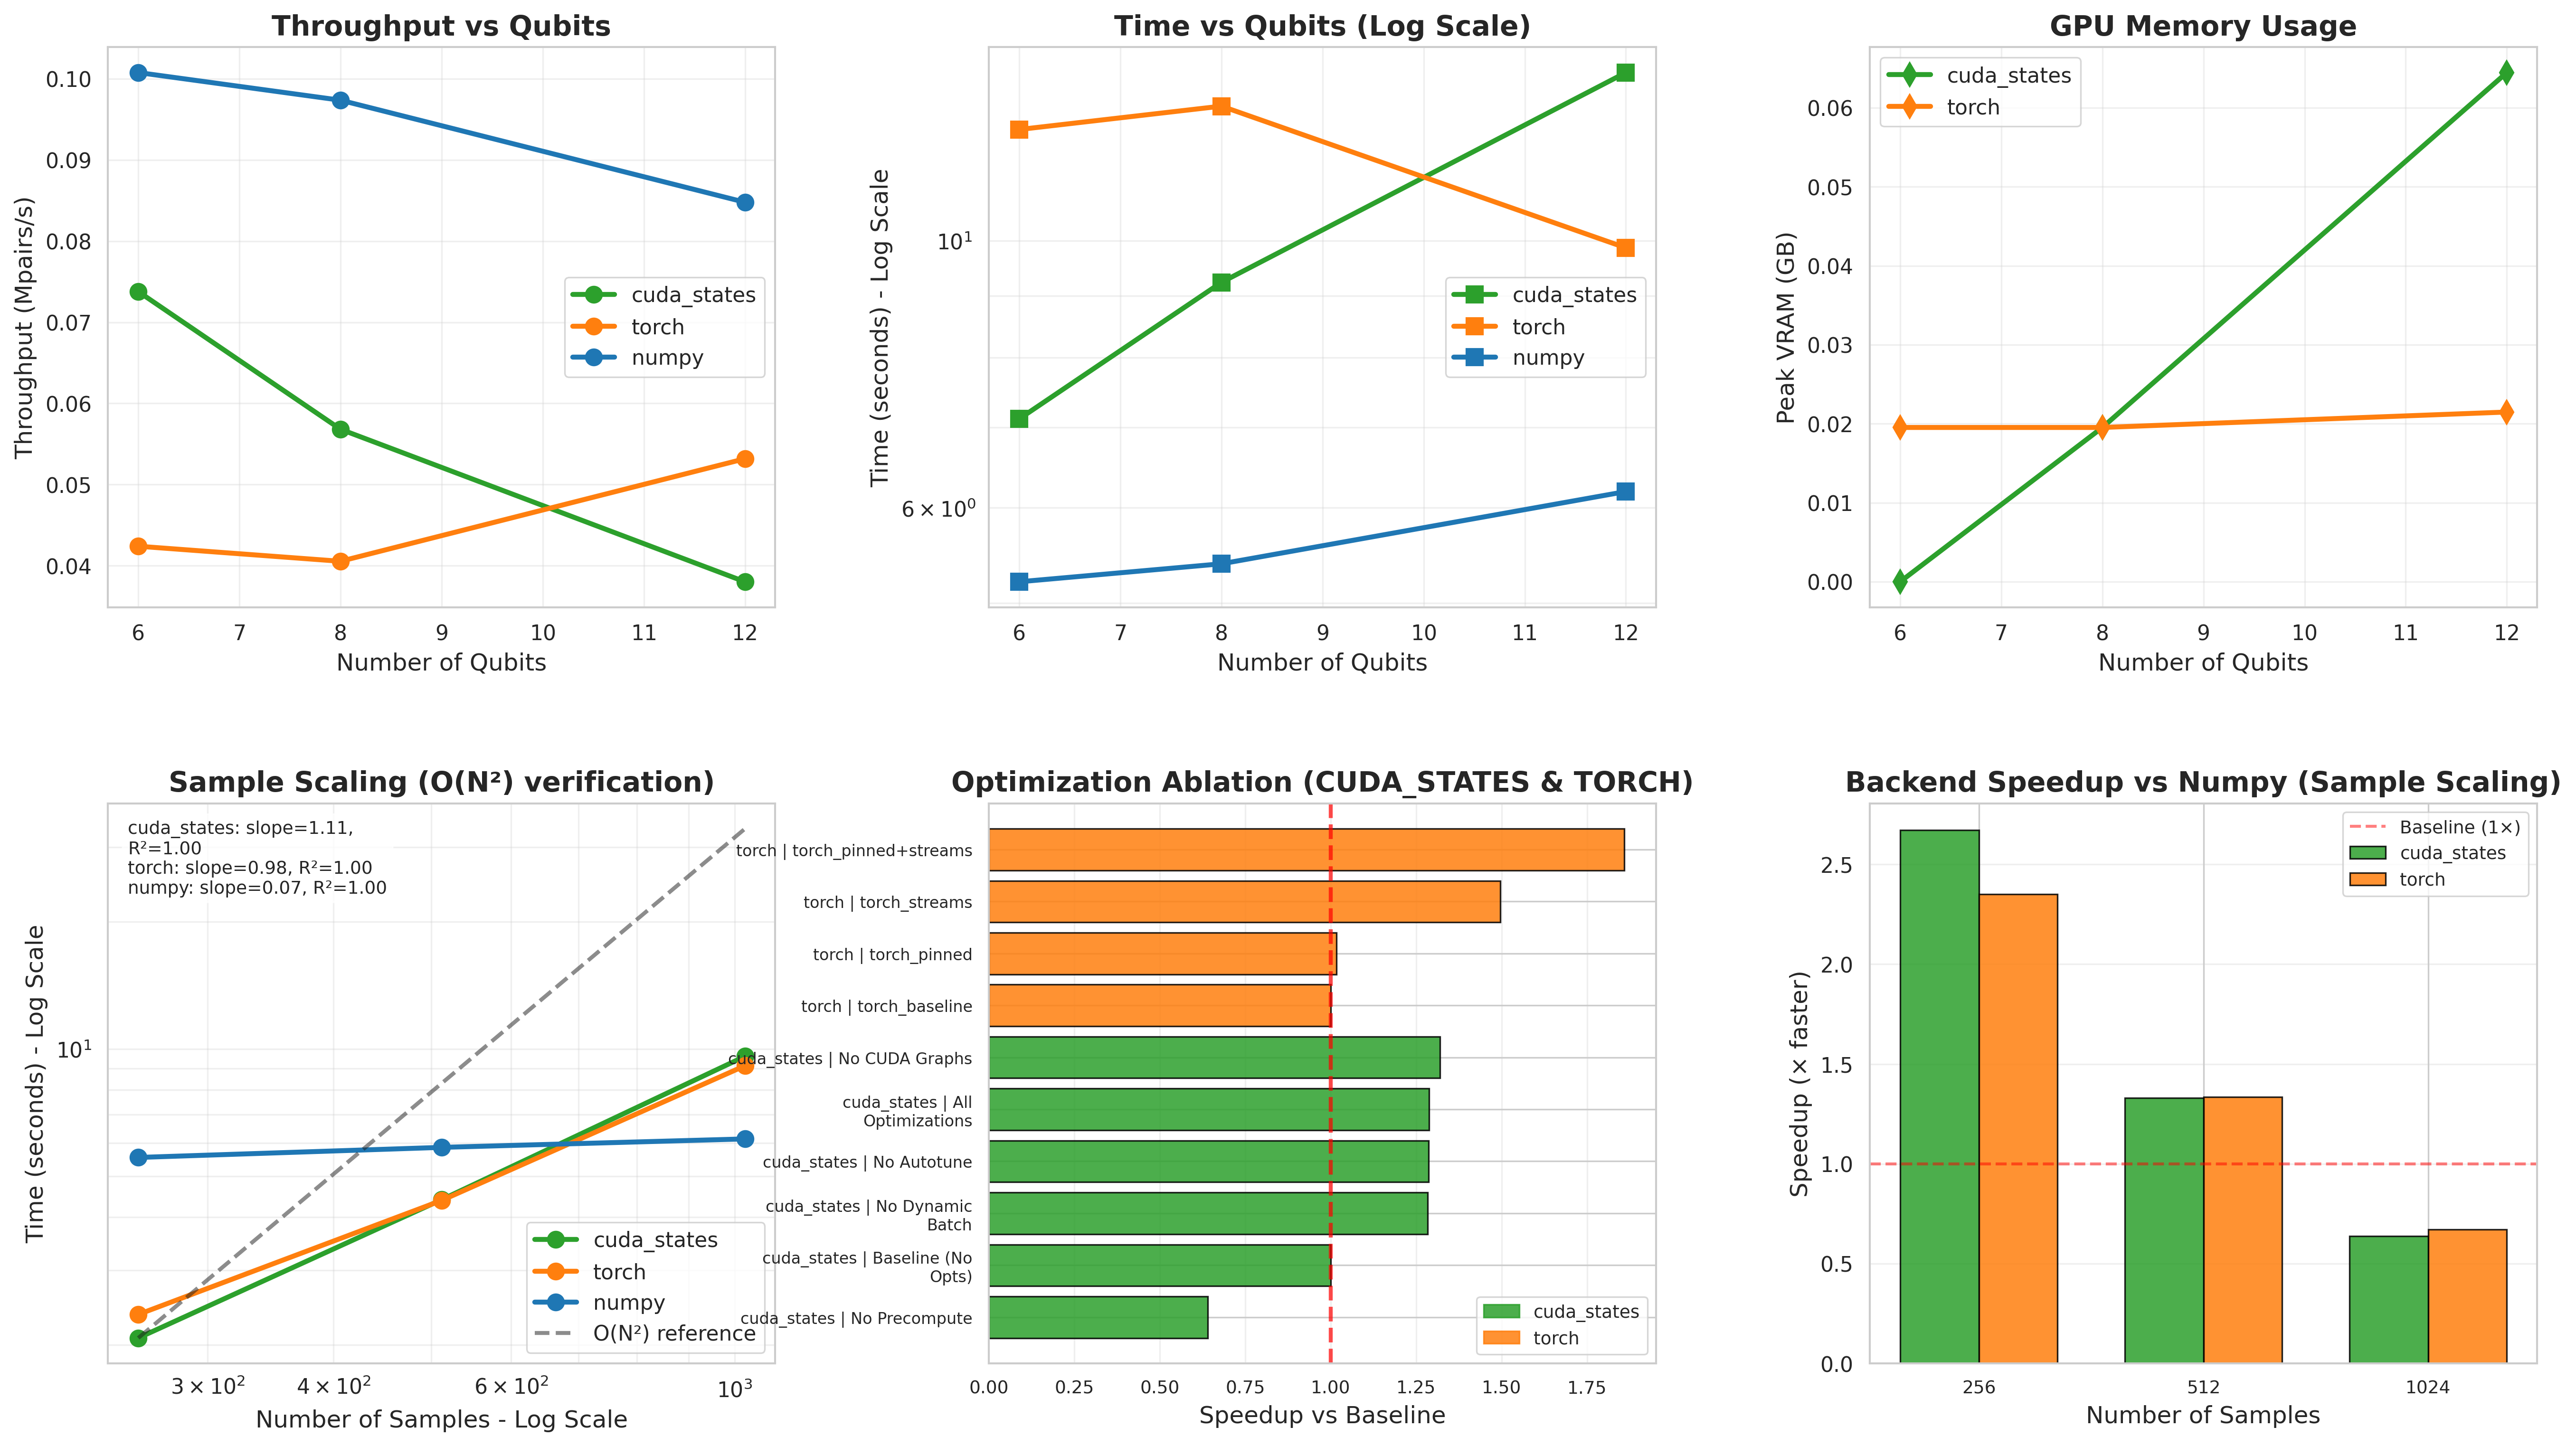
\includegraphics[width=\linewidth]{benchmark_results/fashion/benchmark.png}
    \caption{Fashion-MNIST profile benchmark.}
\end{subfigure}
\hfill
\begin{subfigure}[t]{0.32\textwidth}
    \centering
    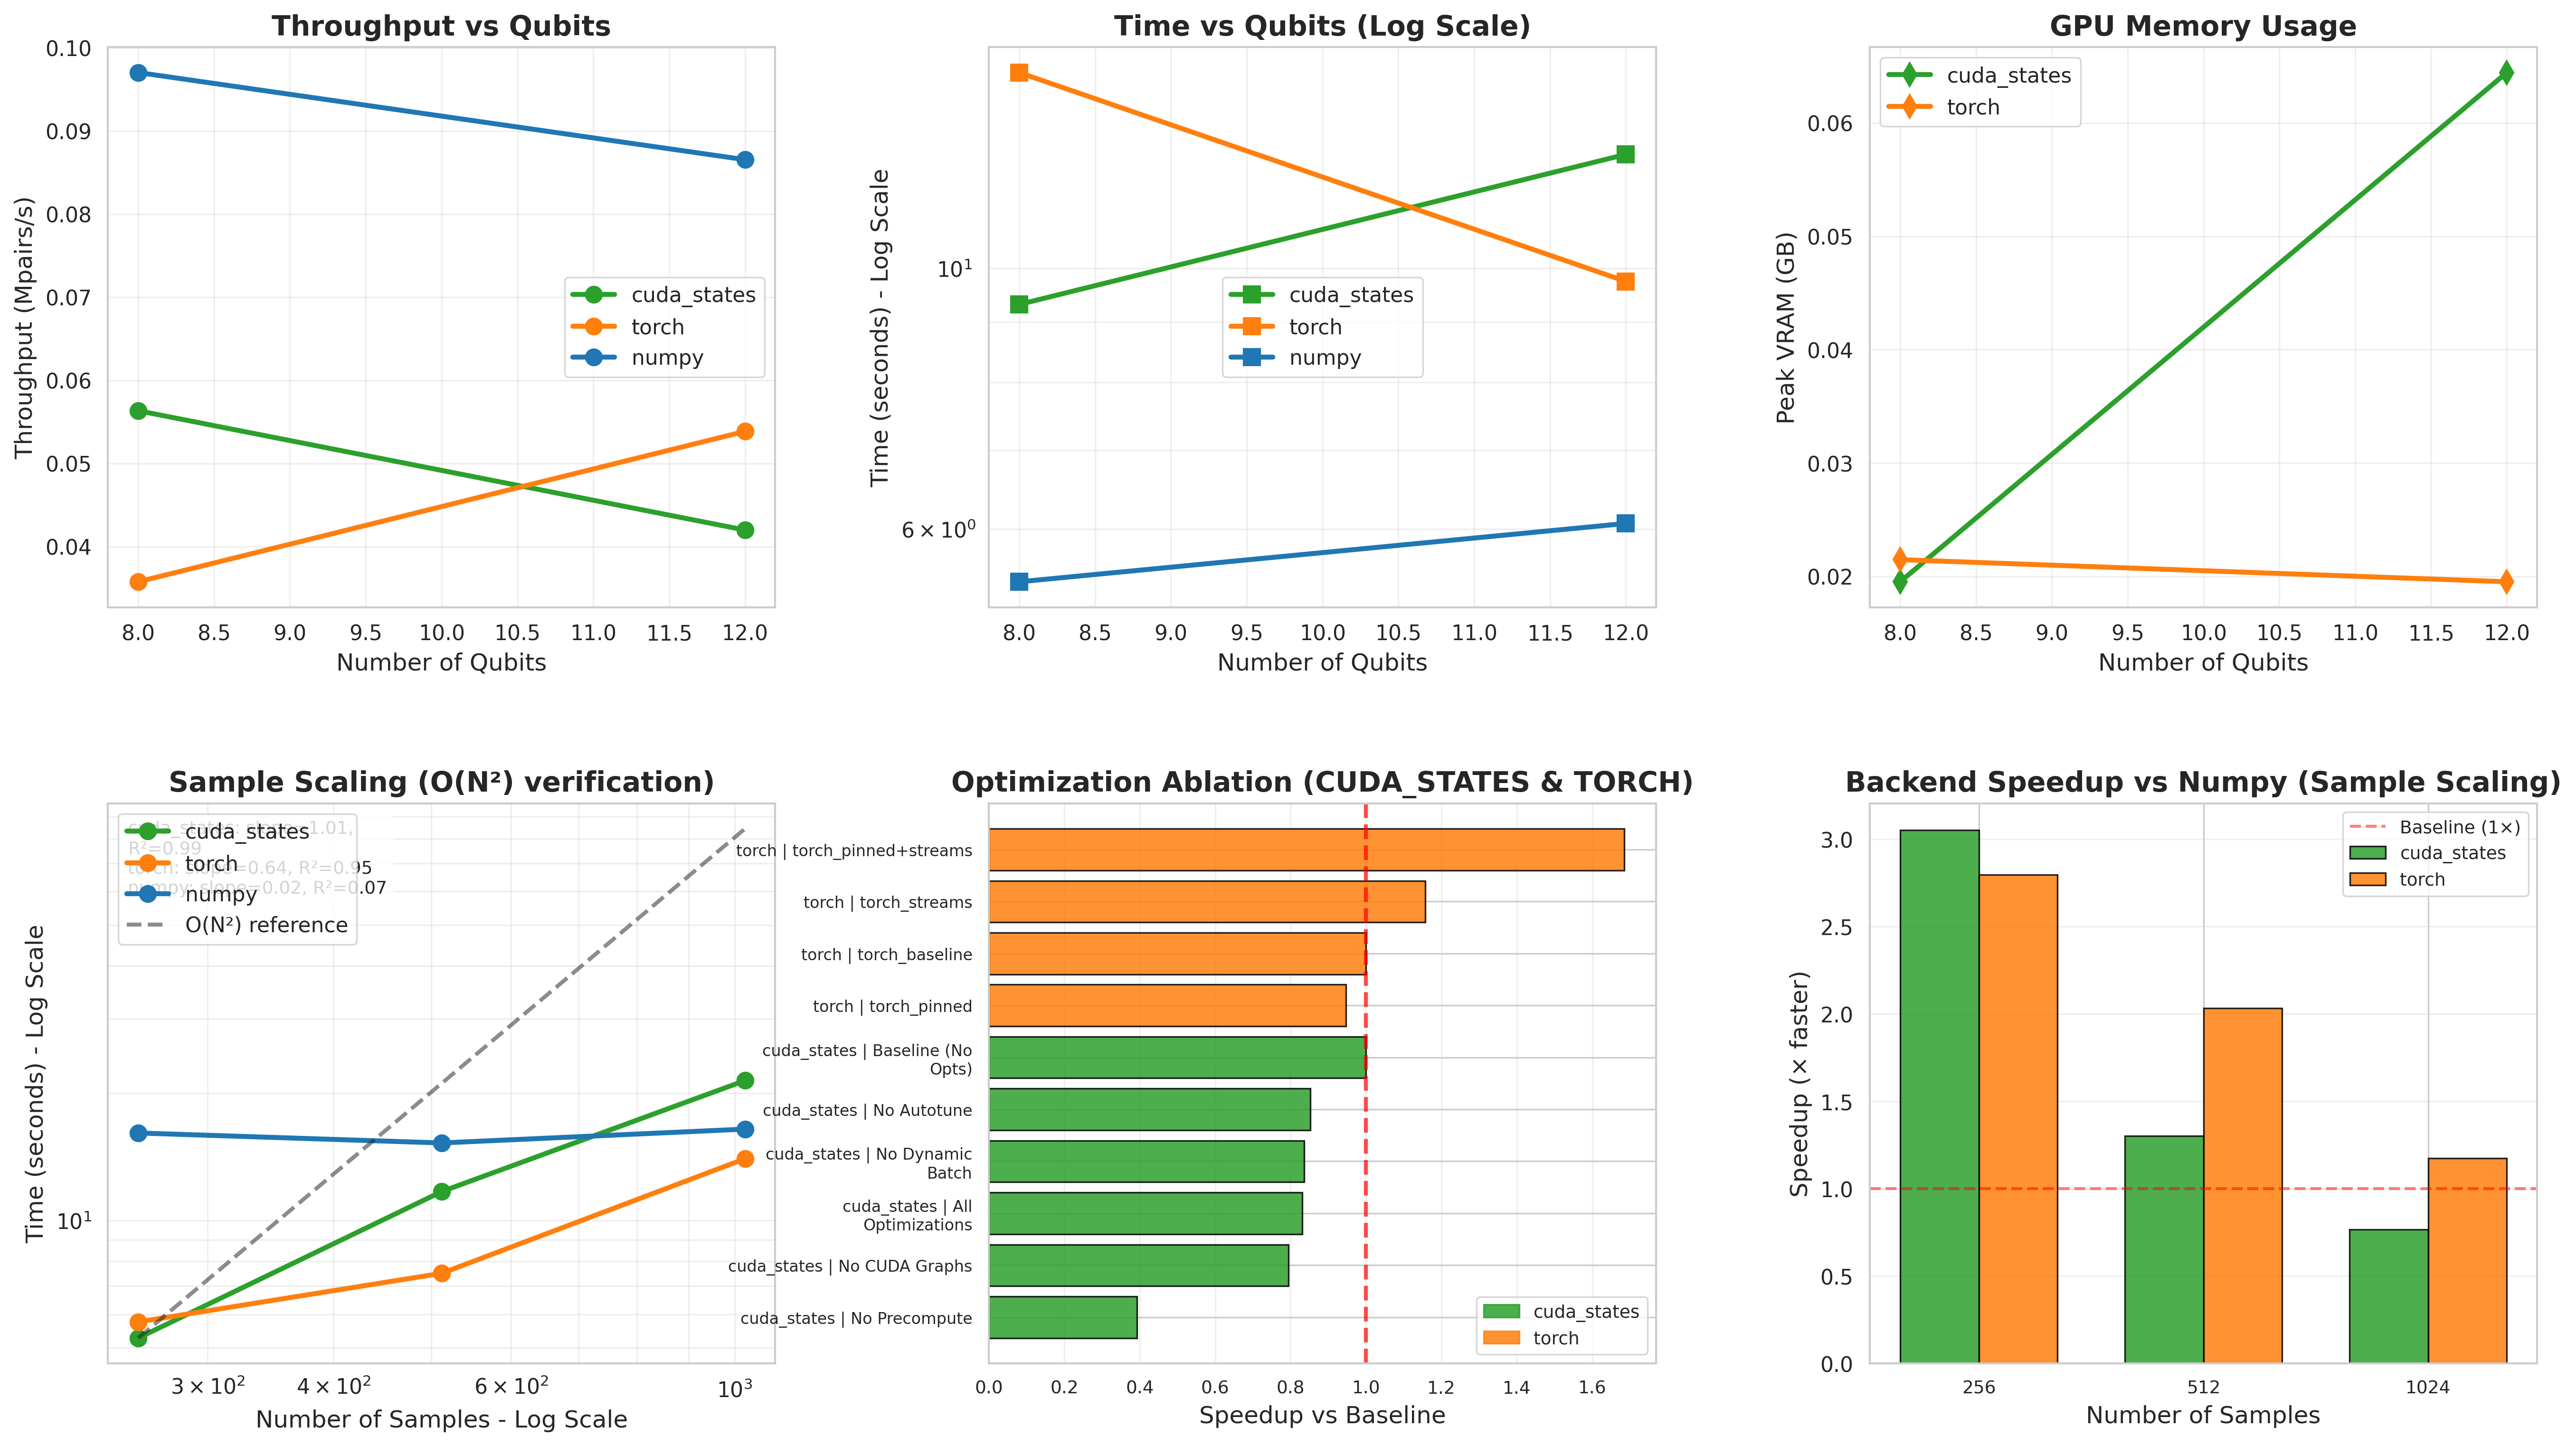
\includegraphics[width=\linewidth]{benchmark_results/cifar10/benchmark.png}
    \caption{CIFAR-10 profile benchmark.}
\end{subfigure}
\hfill
\begin{subfigure}[t]{0.32\textwidth}
    \centering
    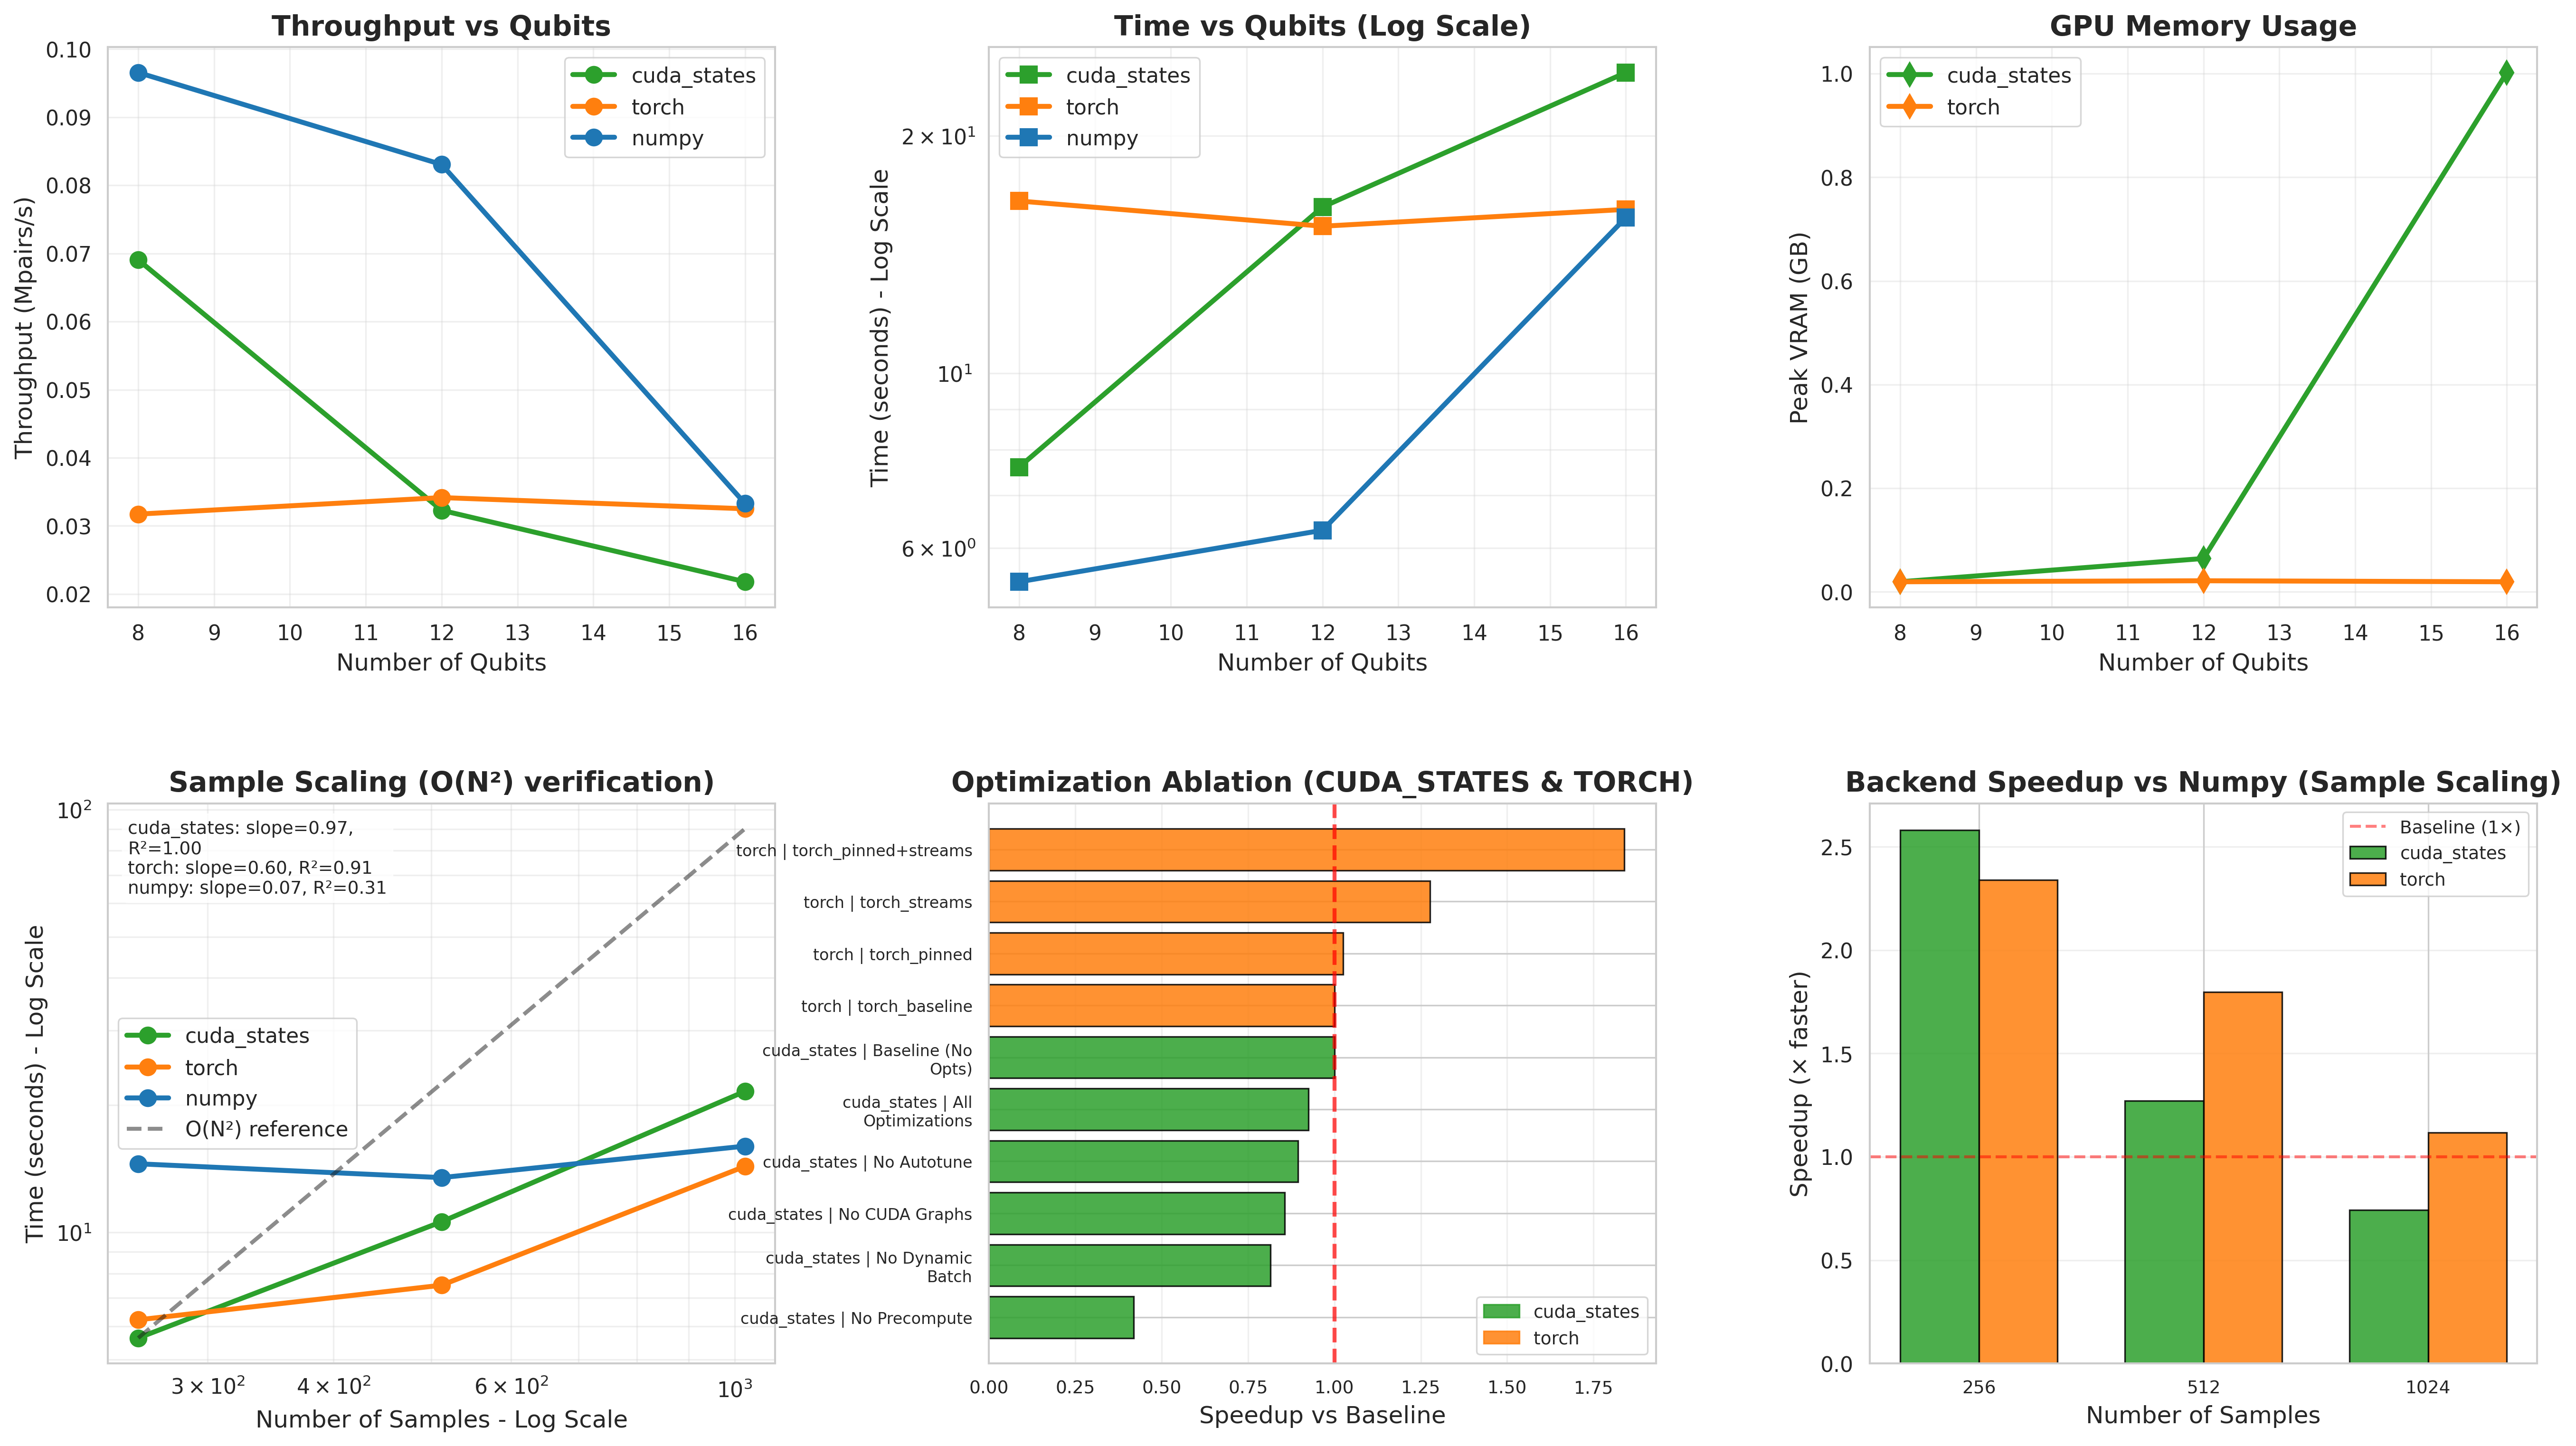
\includegraphics[width=\linewidth]{benchmark_results/svhn/benchmark.png}
    \caption{SVHN profile benchmark.}
\end{subfigure}
\caption{Per-dataset benchmark figures generated by the profile sweep. Each panel includes backend comparison, scaling behavior, optimization ablations, and speedup summaries.}
\label{fig:profile-benchmarks}
\end{figure*}

\subsection{Important Optimization Statistics}
Benchmark ablations identify the most useful settings:
\begin{itemize}
    \item \textbf{Precompute dominates}: disabling precompute is consistently the slowest option.
    \item \textbf{VRAM setting is stable}: \texttt{vram\_fraction=0.95} is best across all three profiles.
    \item \textbf{Stream count is simple}: \texttt{num\_streams=1} is best in the measured sweeps.
    \item \textbf{Torch variant is stable}: \texttt{torch\_pinned+streams} is the strongest torch configuration in all profiles.
\end{itemize}

At this scale, data movement and memory organization have a larger effect than increasing stream complexity.

\section{Classification Results}
\begin{table}[t]
\centering
\caption{Mean classification and runtime statistics on the latest shared setup (sizes 500 and 1000, 18 matched tasks), using \texttt{summary\_results\_latest\_alias.csv} and \texttt{summary\_results\_classical\_20260615\_182830.csv}.}
\label{tab:classification-summary}
\small
\begin{tabular}{lccc}
\toprule
\textbf{Backend} & \textbf{Mean F1} & \textbf{Mean AUC} & \textbf{Mean time/task (min)} \\
\midrule
classical & 0.7120 & 0.8051 & 0.24 \\
torch & 0.5405 & 0.6507 & 4.09 \\
cuda\_states & 0.4842 & 0.6255 & 7.20 \\
\bottomrule
\end{tabular}
\end{table}

The central pattern is that the classical baseline leads in both quality and runtime on the aggregated workload, while torch remains stronger than \texttt{cuda\_states} among the quantum backends.

At dataset level, Fashion-MNIST remains the favorable case for quantum kernels in the latest campaign, whereas CIFAR-10 and especially SVHN show lower AUC and weaker class separation.

\subsection{Latest Run-Scoped Comparison Against the Classical Baseline}
To avoid mixing historical logs, run-scoped summaries are filtered with \texttt{--run} or \texttt{--latest-run}. The latest quantum campaign (36 successful runs) is compared against the latest classical campaign (45 successful runs) on the shared setup (same dataset, difficulty, and sample sizes 500/1000).

The paired analysis is exported in \texttt{summary\_comparison\_by\_dataset\_difficulty.csv}. Table~\ref{tab:latest-run-comparison} reports the aggregate outcome.

\begin{table}[t]
\centering
\caption{Run-scoped paired comparison on shared settings (sizes 500 and 1000). Positive deltas indicate better classical quality; negative time deltas indicate faster classical execution.}
\label{tab:latest-run-comparison}
\small
\begin{tabular}{lccc}
\toprule
\textbf{Comparison} & $\Delta$\textbf{F1} & $\Delta$\textbf{AUC} & $\Delta$\textbf{Time (s)} \\
\midrule
Classical $-$ Torch & +0.1714 & +0.1544 & -231.40 \\
Classical $-$ cuda\_states & +0.2277 & +0.1795 & -417.71 \\
\bottomrule
\end{tabular}
\end{table}

In paired wins, classical records \textbf{16/1/1} against Torch and \textbf{16/1/1} against \texttt{cuda\_states}, confirming the aggregate result in Table~\ref{tab:classification-summary}.

\section{Failure Analysis: Kernel Collapse and Barren Plateau-Like Regimes}
Hard tasks exhibit the following quantitative pattern:
\begin{itemize}
    \item inter-class gap near zero after centering/normalization;
    \item test-kernel standard deviation on the order of $10^{-4}$ to $10^{-3}$;
    \item support-vector fraction near $1.0$;
    \item AUC close to random in the hardest cases.
\end{itemize}

The \texttt{cifar10\_hard} case with \textbf{6 layers} is particularly revealing. In logs such as \texttt{log\_cifar10\_hard\_torch\_500\_6layers.txt} one typically observes:
\begin{itemize}
    \item \texttt{Val kernel std = 0.0005};
    \item \texttt{support\_frac = 1.0000};
    \item \texttt{test\_F1 = 0.0000};
    \item \texttt{test\_AUC = 0.4757}.
\end{itemize}

This behavior is consistent with a \textbf{kernel concentration}: states become almost indistinguishable in terms of overlap used by the SVM. It is reasonable to interpret this as a \emph{barren-plateau-like} or \emph{kernel collapse} regime~\cite{larocca2024review,thanasilp2022exponential}, although multiple factors likely combine:
\begin{itemize}
    \item loss of information due to conversion to grayscale and subsequent PCA;
    \item generic ansatz not informed by image geometry;
    \item increased depth favoring concentration of overlaps;
    \item intrinsic limitations of global fidelity kernels on complex visual data.
\end{itemize}

These observations indicate that compute acceleration alone does not resolve representational limits of the feature map.

\section{Reproducibility and Engineering Hygiene}
Reproducibility is supported by containerized execution and run-scoped extraction:
\begin{itemize}
    \item same software environment for all runs;
    \item explicit separation of classical and quantum sweeps;
    \item deterministic run filtering with \texttt{--run} and \texttt{--latest-run};
    \item persistent caches for kernels and autotune settings.
\end{itemize}

\subsection{Minimal Reproducibility Workflow}
The minimal command sequence to reproduce the quantum training campaign is:
\begin{enumerate}
    \item Build the GPU Docker image:\\{\small\texttt{docker compose build trainer-quantum}}
    \item Launch the quantum sweep on available GPUs:\\{\small\texttt{bash run\_all\_quantum.sh}}
    \item Launch the classical baseline:\\{\small\texttt{bash run\_all\_classical.sh}}
    \item Extract results from the latest run only:\\{\small\texttt{docker compose run --rm extract-results python3 extract\_results.py --latest-run --csv summary\_results\_latest.csv}}
    \item Extract a specific timestamped run:\\{\small\texttt{docker compose run --rm extract-results python3 extract\_results.py --run 20260615\_211954}}
\end{enumerate}

The \texttt{--latest-run} flag introduced in \texttt{extract\_results.py} prevents mixing logs from different historical runs. The \texttt{summary\_comparison\_by\_dataset\_difficulty.csv} artifact consolidates paired classical-vs-quantum deltas across all dataset/difficulty/size combinations.

\section{Data and Code Availability}
The full project repository is publicly available at:\\{\small\url{https://github.com/DylanUnifi/ProjectWorkParallelProgramming}}

Datasets are loaded automatically from standard sources:
\begin{itemize}
    \item \textbf{Fashion-MNIST}~\cite{xiao2017fashion}: via \texttt{torchvision.datasets.FashionMNIST}.
    \item \textbf{CIFAR-10}~\cite{krizhevsky2009cifar}: via \texttt{torchvision.datasets.CIFAR10}.
    \item \textbf{SVHN}~\cite{netzer2011svhn}: via \texttt{torchvision.datasets.SVHN}.
\end{itemize}

Key artifacts generated by the experiments and referenced in this report:
\begin{itemize}
    \item \texttt{summary\_results\_latest\_alias.csv} and \texttt{summary\_results\_classical\_20260615\_182830.csv} — latest run-scoped results used for Table~\ref{tab:classification-summary}.
    \item \texttt{summary\_comparison\_by\_dataset\_difficulty.csv} — run-scoped paired deltas (Table~\ref{tab:latest-run-comparison}).
    \item \texttt{benchmark\_results/benchmark.csv} — backend throughput data (Table~\ref{tab:benchmark}).
    \item \texttt{benchmark\_results/\{fashion,cifar10,svhn\}/benchmark.png} — profile benchmark figures (Fig.~\ref{fig:profile-benchmarks}).
    \item \texttt{.cuda\_kernel\_autotune.json} — persistent CUDA tile autotune cache.
\end{itemize}

\section{Conclusion}
The measured results show a consistent trade-off. Classical SVM remains strongest on aggregated quality and runtime, while \texttt{cuda\_states} leads direct backend throughput panels on the benchmark profiles.

Simulated quantum kernels stay competitive on easier distributions (notably Fashion-MNIST), but performance degrades on CIFAR-10 and SVHN where kernel concentration indicators are strongest. This points to feature-map expressivity as the primary bottleneck beyond raw compute efficiency.

\section{Perspectives}
Data-supported next steps are:
\begin{itemize}
    \item projected or local kernels to limit global fidelity concentration;
    \item geometry-aware ansatzes for image data;
    \item systematic comparison with stronger classical features before PCA;
    \item multi-GPU or MPI to distribute a single Gram matrix;
    \item scale up cross-benchmarks between \texttt{torch} and \texttt{cuda\_states};
    \item possible integration of a native GPU SVM solver to remove the final CPU bottleneck.
\end{itemize}

{\small
\bibliographystyle{ieeetr}
\bibliography{parallel_qkernel_references}
}

\end{document}
